\section{Microeconomics Midterm 2017 / 18}

{
\subsection*{Schmidt}

{
\subsubsection*{Exercise 1}

\begin{enumerate}[label=(\alph*)]
{\item 
Since $5 \in[0,7.5]$, this violates WARP. 

See below in ex (b) why this is true.
}
{\item 
To violate WARP must find:

$$
\left|\begin{array}{l}
p^{\prime} x \leq w^{\prime} \\
p x^{\prime} \leq w
\end{array}\right|
$$

Note that we find $w$ \& $w^{\prime}$ by Walras Law:

$$
\begin{aligned}
& \left|\begin{array}{l}
2 \cdot 10+4 \cdot y \leq 50 \\
6 \cdot 5+3 \cdot 10 \leq 60+3 \cdot y
\end{array}\right| \\
& \Leftrightarrow \left\lvert\, \begin{aligned}
20+4 y & \leqslant 50 \\
60 & \leqslant 60+3 y \mid
\end{aligned}\right. \\
& \Longleftrightarrow\left|\begin{array}{l}
y \leqslant 7.5 \\
0 \leqslant y
\end{array}\right|
\end{aligned}
$$

Thus WARP is violated if $y \in[0,7.5]$.
}
\end{enumerate}
}
{
\subsubsection*{Exercise 2}

\begin{enumerate}[label=(\alph*)]
{\item 
Budget constraint:

$$
\begin{aligned}
p x_{1}+x_{2} & =w \quad \mid \text { use } x_{1}=\frac{1}{p} \\
\Leftrightarrow \quad x_{2} & =w-1
\end{aligned}
$$
}
{\item 
This has to be quasi-lineor:

$$
\begin{aligned}
v(p, w) & =f\left(x_{1}(p, w)\right)+x_{2}(p, w) \\
& =f\left(\frac{1}{p}\right)+w-1
\end{aligned}
$$

By Roy's identity:

$$
\begin{array}{lcl}
x_{1}= & -\frac{\frac{\partial v\left(p_{n}\right)}{\partial p}}{\frac{\partial v}{\partial w}}=-\frac{f^{\prime}\left(\frac{1}{p}\right)(-1)\left(\frac{1}{p}\right)^{2}}{1} \stackrel{!}{=} & \frac{1}{p} \\
\Leftrightarrow & f^{\prime}\left(\frac{1}{p}\right)=p & \text { use } p=\frac{1}{x_{1}} \\
\Leftrightarrow & f^{\prime}\left(x_{1}\right)=\frac{1}{x_{1}} \\
\Leftrightarrow & \int_{\underline{x}_{1}}^{x_{1}} f^{\prime}(t) d t=\int_{\underline{x}_{1}}^{x_{1}} \frac{1}{t} d t
\end{array}
$$
$\Longleftrightarrow \quad f\left(x_{1}\right)-f\left(\underline{x}_{1}\right)=\ln \left(x_{1}\right)-\ln \left(\underline{x}_{1}\right)$

Thus:

$$
f\left(x_{1}\right)=\ln \left(x_{1}\right)+\alpha
$$

For simplicity, let $\alpha=0$, as utility is ordinal. Find:

$$
v(p, w)=\ln \left(\frac{1}{p}\right)+w-1
$$
}
{\item 
 Immediately from (b):

$$
u\left(x_{1}, x_{2}\right)=\ln \left(x_{1}\right)+x_{2}
$$
}
\end{enumerate}
}
{
\subsubsection*{Exercise 3}

Cash constraints turn this problem into a consumer problem.

\begin{enumerate}[label=(\alph*)]
{\item 
Treat $R(\cdot)$ as indirect utility \& $C$ as wealth.

Apply Roy's identity:

$$
z_{1}\left(p_{1} w_{1}, w_{2}\right)=-\frac{\frac{\partial R(\cdot)}{\partial w_{1}(\cdot)}}{\frac{\partial R}{\partial C}}=-\frac{p(-\alpha) 1 / w_{1}}{p \cdot 1 / C}=\alpha \frac{C}{w_{1}}
$$
}
{\item
Invert $R(\cdot)$ to find $C(\cdot)$ :

\begin{align*}
    & \frac{R}{p}=\gamma+\ln \left[\frac{C}{w_{1}^{\alpha} w_{2}^{1-\alpha}}\right] \\
    & \Leftrightarrow \quad \exp \left[\frac{R}{P}-\gamma\right]=\frac{C}{w_{1}^{\alpha} w_{2}^{1-\alpha}} \\
    & \Leftrightarrow C\left(p, w_{1}, w_{2}\right)=w_{1}^{\alpha} w_{2}^{1-\alpha} \exp \left[\frac{R}{p}-\gamma\right] \tag{I}
\end{align*}
}
{\item 
Apply Shepherd's Lemma to (I):

$$
\tilde{z}_{1}\left(p_{1} w_{1}, w_{2}\right)=\frac{\partial C(\cdot)}{\partial w_{1}}=\alpha\left(\frac{w_{2}}{w_{1}}\right)^{1-\alpha} \exp \left[\frac{R}{p}-\gamma\right]
$$
}
\end{enumerate}
}
{
\subsubsection*{Exercise 4}

\begin{enumerate}[label=(\alph*)]
{\item 
(1) risk aversion: $u^{\prime \prime}(x)=2 c<0 \Longleftrightarrow c<0$

(2) marginal utility must be positive:

$$
\begin{array}{rlrl} 
    u^{\prime}(x)=b+2 c x & >0 \\
    \Rightarrow \quad b & >2 x|c|
\end{array}
$$

There is no restriction on $a$. $a$ only shifts the utility up or down.
}
{\item 
To satisfy (2) from (a), must have

$$
x \in\left[0,-\frac{b}{2 c}\right]
$$
}
{\item 
$$
\begin{aligned}
E U(x) & =\int a+b x+c x^{2} d F(x) \\
& =a+b \int x d F(x)+c \int x^{2} d F(x) \\
& =a+b \mathbb{E}(x)+c \mathbb{E}\left(x^{2}\right) \quad \mid \text { let } \mathbb{E}(x)=\mu \text{ and } Var(x) = \sigma^2\\
& =a+b \mu+c\left(\sigma^{2}+\mu^{2}\right)
\end{aligned}
$$
}
{\item 
$$
\max _{s} \int a+b(w-s+s r)+c(w-s+s r)^{2} d F(r)
$$

Note: 

$$
\begin{aligned}
    \mathbb{E}(w-s+s r)=w-s+s \mathbb{E}(r)=w-s+s \mu r \\
    \operatorname{Var}(w-s+s r)=s^{2} \operatorname{Var}(r)=s^{2} G_{r}^{2}
\end{aligned}
$$

Thus:

\begin{align*}
\max _s a+b\left(w-s+s \mu_r\right)+c\left[s^2 G_r^2+\left(w-s+s \mu_r\right)^2\right]
\end{align*}

FOC:

\begin{align*}
    & b\left(\mu_r-1\right)+c 2\left[s G_r^2+\left(w-s+s \mu_r\right)\left(\mu_r-1\right)\right]=0 \\
    & s G_r^2+\omega\left(\mu_r-1\right)+s\left(\mu_r-1\right)^2=\left(1-\mu_r\right) \frac{b}{2 c} \\
    & s\left[\sigma_r^2+\left(\mu_r-1\right)^2\right]=\left(1-\mu_r\right)\left(\frac{b}{2 c}+\omega\right)
\end{align*}

\begin{align*}
s^*=\frac{\left(1-\mu_r\right)\left(\frac{b}{2 c}+\omega\right)}{\sigma_r^2+\left(\mu_r-1\right)^2}
\end{align*}

and therefore we find that

\begin{align*}
\frac{\partial s^*}{\partial w}=\frac{1-\mu_r}{\sigma_r^2+\left(\mu_r-1\right)^2}<0
\end{align*}
}
\end{enumerate}
}
}

{
\subsection*{Gottardi}

{
\subsubsection*{Exercise 1}

\begin{enumerate}[label=(\alph*)]
{\item Figure says it all 

\begin{figure}[!htp]
    \centering
    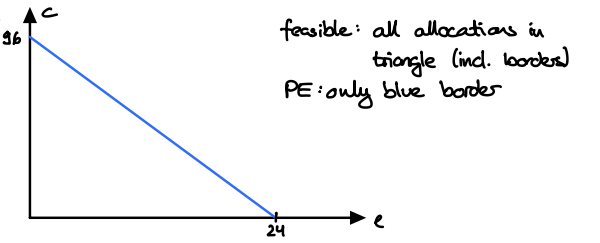
\includegraphics[width=.75\textwidth]{images/2017_18_1.png}
\end{figure}
}
{\item 
\underline{Consumer:}

\begin{align*}
    \max_{c,l} cl \\
    \text{s.t. } pc+w l=w 24 \\
    \Longleftrightarrow \max _{c} c\left[24-\frac{p}{w c}\right]
\end{align*}

FOC: 

\begin{align*}
    24-2 \frac{P}{w c}=0 \\
    \Leftrightarrow \quad c=12(p / w)^{-1}
\end{align*}

\underline{Firm:}

\begin{align*}
    \max_L p 4 L-w L=\max_L L\left(4p-w\right)
\end{align*}

$$
L=\left\{\begin{array}{lll}
\infty & \text { if } & p / w>1 / 4 \\
\mathbb{R}^{+} & \text {if } & p / w=1 / 4 \\
0 & \text { if } & p / w<1 / 4
\end{array}\right.
$$

\underline{Markets:}

To clear labour market, must have $p / w=1 / 4$ or there will be excess demand or supply.

$$
\longrightarrow c=12(p / w)^{-1}=48
$$

to clear goods market: $c=y=48$

$$
\longrightarrow l=24-\frac{p}{w} c=12
$$

by labour market: $L=24-l=12$

\underline{Competitive Equlibrium:}

\begin{align*}
    \frac{p}{w}=\frac{1}{4} ; y=48 ; L=12
\end{align*}

This allocation is $P E$ as it is on the border of the blue triangle described by

$$
c=24-\frac{1}{4} l
$$
}
{\item 
The price ratio is the same or labour market cannot clear.

\underline{Consumer:}

$$
\begin{aligned}
& \max _{c, l} c l-\bar{y} \\
& \text { s.t. } \bar{y}=4(24-l) \\
& p c+w l=24 w \\
& \Leftrightarrow \max _{l}\left(24(p / w)^{-1}-l(p / w)^{-1}\right) l-4(24-l)
\end{aligned}
$$

FOC:

$$
\begin{aligned}
& 24(p / w)^{-1}-2 l(p / w)^{-1}+4=0 \\
& 12+1-l=0 \\
& l=13
\end{aligned}
$$

\underline{Markets:}

$$
\begin{aligned}
& L=24-l=11 \\
& c=y=44
\end{aligned}
$$

\underline{Competitive Equilibrium:}

$$
\frac{p}{w}=\frac{1}{4} ; L=11 ; y=44
$$

This is not PE anymore.
}
\end{enumerate}
}
{
\subsubsection*{Exercise 2}

No. Only need LNS by FWT. But without convexity we may not have a CE at all.
}
{
\subsubsection*{Exercise 3}

\begin{enumerate}[label=(\alph*)]
{\item 
$$
\begin{array}{ll}
t=0: & q_{1} \theta_{1}+q_{2} \theta_{2}=0 \\
t=1\: ; \:s=1: & x_{1}=\theta_{1}+8 \\
t=1\: ; \:s=2: & x_{2}=\theta_{2}+2
\end{array}
$$

Combine:

$$
q_{1}\left(x_{1}-8\right)+q_{2}\left(x_{2}-2\right)=0
$$
}
{\item 
$$
\begin{gathered}
\max _{x_{1}, x_{2}} \frac{1}{2}\left[10 x_{1}-\frac{1}{2} x_{1}^{2}+10 x_{2}-\frac{1}{2} x_{2}^{2}\right] \\
\text { s.t. } q_{1}\left(x_{1}-8\right)+q_{2}\left(x_{2}-2\right)=0
\end{gathered}
$$

FOCs:

$$
\begin{gathered}
\left[x_{1}\right]: \quad \frac{1}{2}\left(10-x_{1}\right)-\lambda q_{1}=0 \\
{\left[x_{2}\right]: \quad \frac{1}{2}\left(10-x_{2}\right)-\lambda q_{2}=0}
\end{gathered}
$$

Combine FOCs:

$$
\frac{q_{1}}{q_{2}}=\frac{10-x_{1}}{10-x_{2}}
$$

Asset market clearing implies $\theta_{1}=\theta_{2}=0$ as there is only one consumer. As a result: $x_{1}=w_{1}$ and $x_{2}=w_{2}$.

$$
\frac{q_{1}}{q_{2}}=\frac{10-8}{10-2}=\frac{2}{8}=\frac{1}{4}
$$

We find $q_{1}<q_{2}$, although $\mathbb{E}\left(r_{1}\right)=\mathbb{E}\left(r_{2}\right)=1 / 2$. The reason is that the risk averse consumer wants to insure against the poor state (2) by buying asset 2. But as she is alone this creates excess demand for asset 2. This drives the price up until the consumer does not want to boy or sell.
}
{\item 
No. By removing risk aversion, the prices will reflect the state probabilities as the consumer only cares about expected payoff. Thus $q_{1}=q_{2}$ and $\frac{q_1}{q_2}=1$.
}
\end{enumerate}
}
}